\section{Deployment}

\begin{frame}{Deployment 1}
    \begin{minipage}[t]{0.35\textwidth}
        Deployment in seperaten Containern mit Docker Compose:
        \begin{itemize}
            \item server
            \begin{itemize} 
                \item API Server
                \item Python + Flask
                \item Deployment mit Gunicorn
            \end{itemize}
            \item app
            \begin{itemize} 
                \item mobile App
                \item Flutter + Dart
                \item Deployment mit nginx
            \end{itemize}
            \item admin
            \begin{itemize} 
                \item Admin Webinterface
                \item REACT
                \item Deployment mit nginx
            \end{itemize}
        \end{itemize}
    \end{minipage}
    \hfill
    \begin{minipage}[t]{0.63\textwidth}
        \begin{figure}
            \begin{center}
                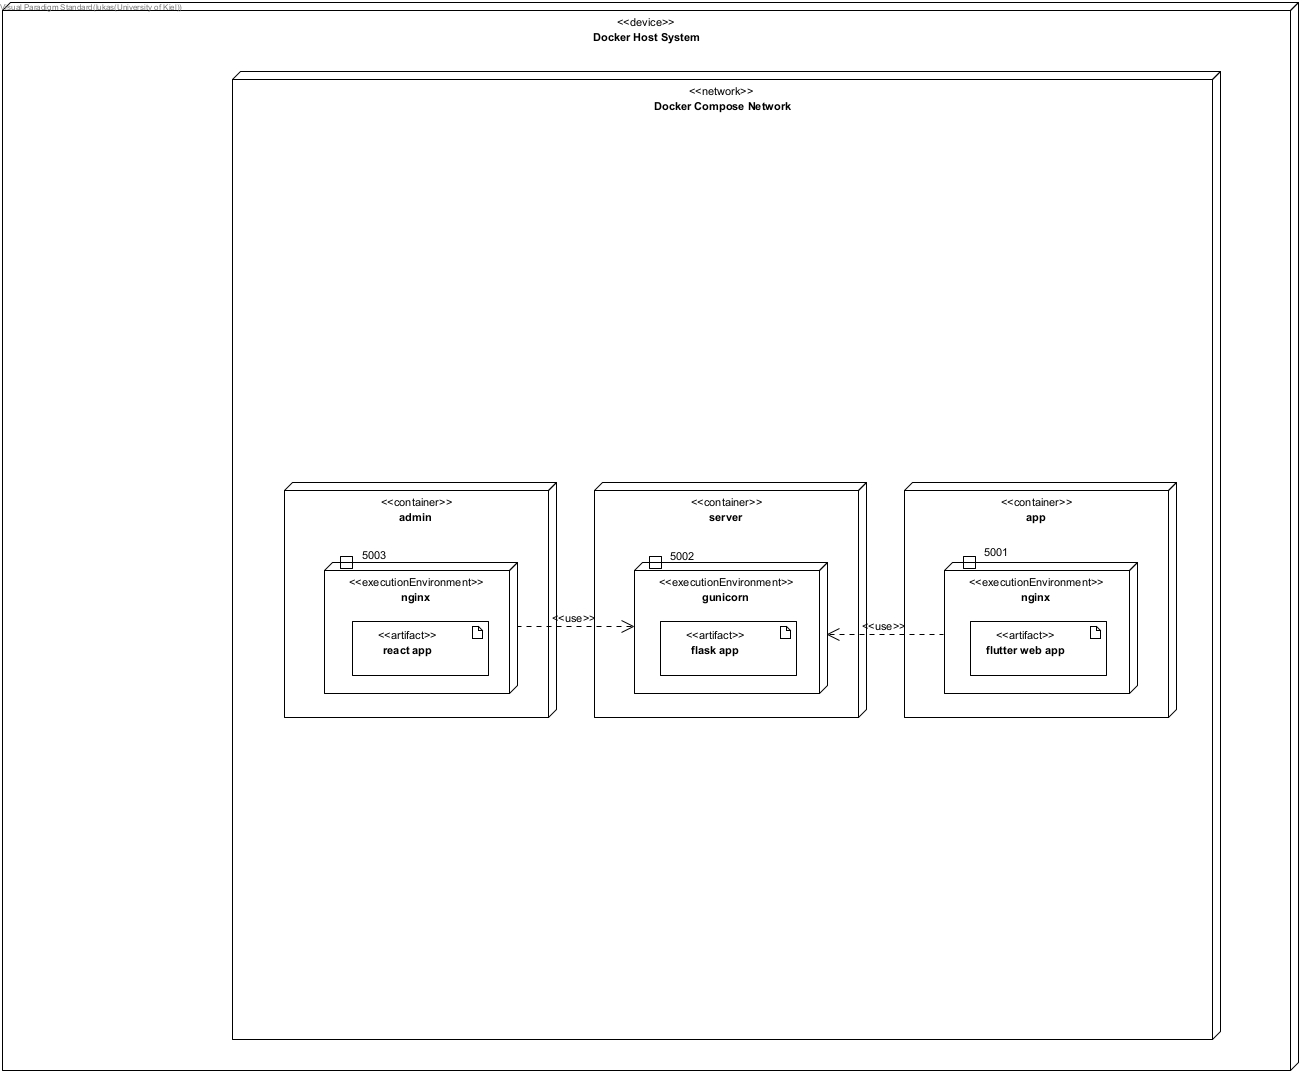
\includegraphics[width=\textwidth]{images/deployment/deployment_diagram_services.jpg}
            \end{center}
        \end{figure}
    \end{minipage}
\end{frame}

\begin{frame}{Deployment 2}
    \begin{minipage}[t]{0.35\textwidth}
        Datenbank:
        \begin{itemize}
            \item PostgreSQL
            \item andere Datenbanken konfigurierbar
            \item Zugriff nur durch API Server
        \end{itemize}
        $ $\\
        Persistenz über Docker Volumes:
        \begin{itemize}
            \item manvsim-db
            \item manvsim-media
        \end{itemize}
    \end{minipage}
    \hfill
    \begin{minipage}[t]{0.63\textwidth}
        \begin{figure}
            \begin{center}
                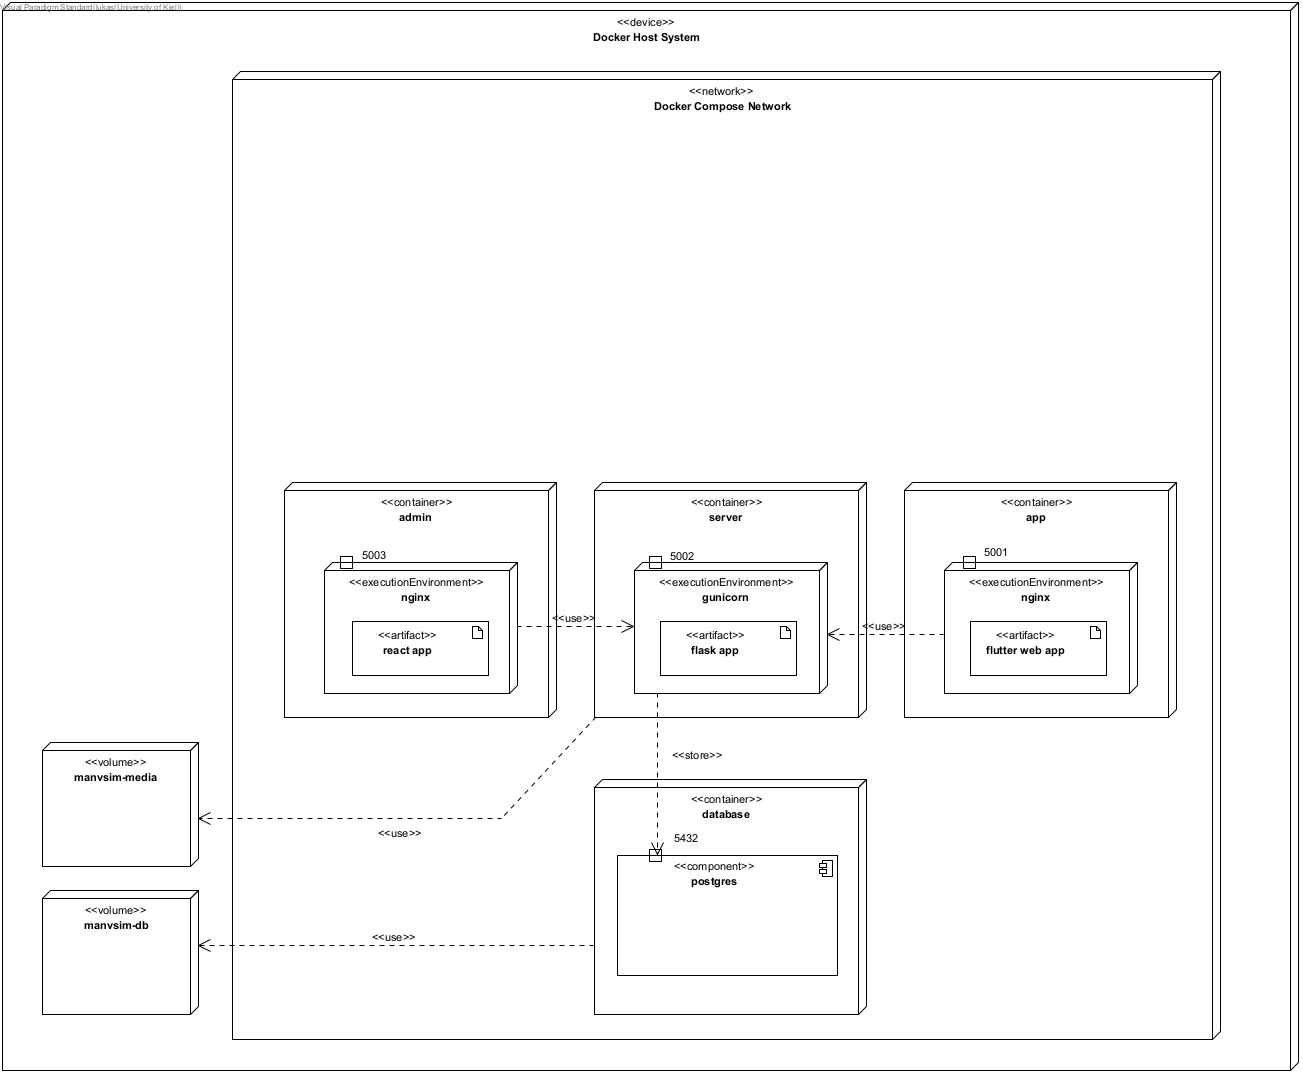
\includegraphics[width=\textwidth]{images/deployment/deployment_diagram_database.jpg}
            \end{center}
        \end{figure}
    \end{minipage}
\end{frame}

\begin{frame}{Deployment 3}
    \begin{minipage}[t]{0.35\textwidth}
        Erreichbarkeit der Container über Reverse Proxy:
        \begin{itemize}
            \item nginx
            \item Deployment von Landing Page
            \item Path based Routing
            \item TLS
            \begin{itemize}
                \item Let's Encrypt Zertifikate über Volume
                \item innerhalb des Docker Netzwerks nur HTTP
            \end{itemize}
            \item Port Freigabe/Mapping
            \begin{itemize}
                \item 80:80 (http)
                \item 443:443 (https)
            \end{itemize}
        \end{itemize}
    \end{minipage}
    \hfill
    \begin{minipage}[t]{0.63\textwidth}
        \begin{figure}
            \begin{center}
                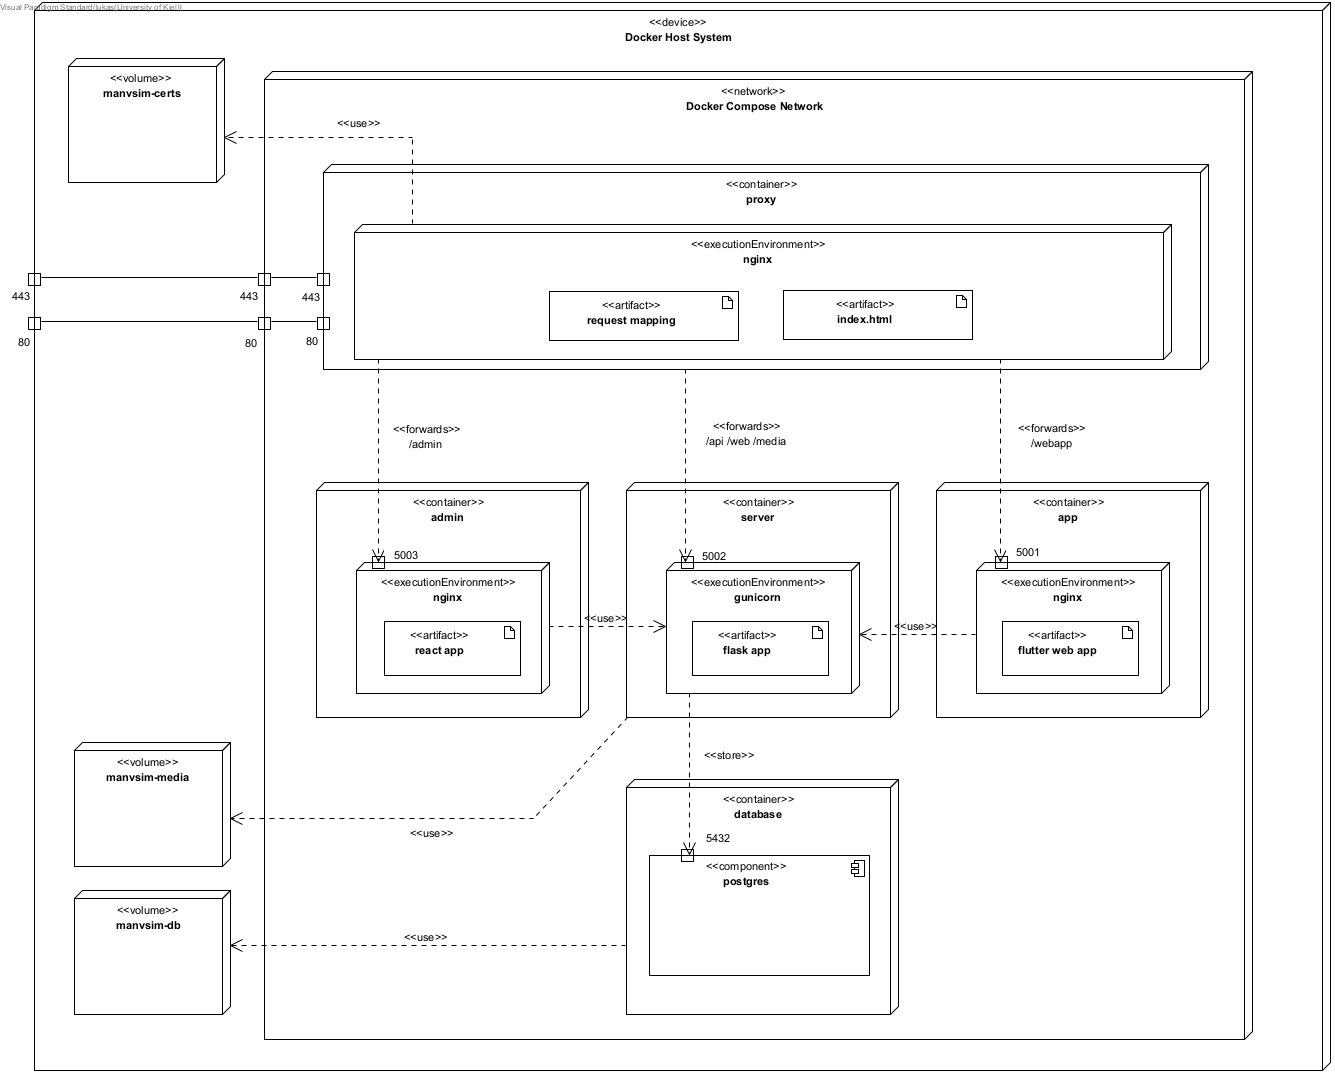
\includegraphics[width=\textwidth]{images/deployment/deployment_diagram_full.jpg}
            \end{center}
        \end{figure}
    \end{minipage}
\end{frame}